\documentclass[border=5mm]{standalone}
\usepackage{pgfplots}
\pgfplotsset{compat=1.18}
\usetikzlibrary{decorations.pathreplacing}

\begin{document}
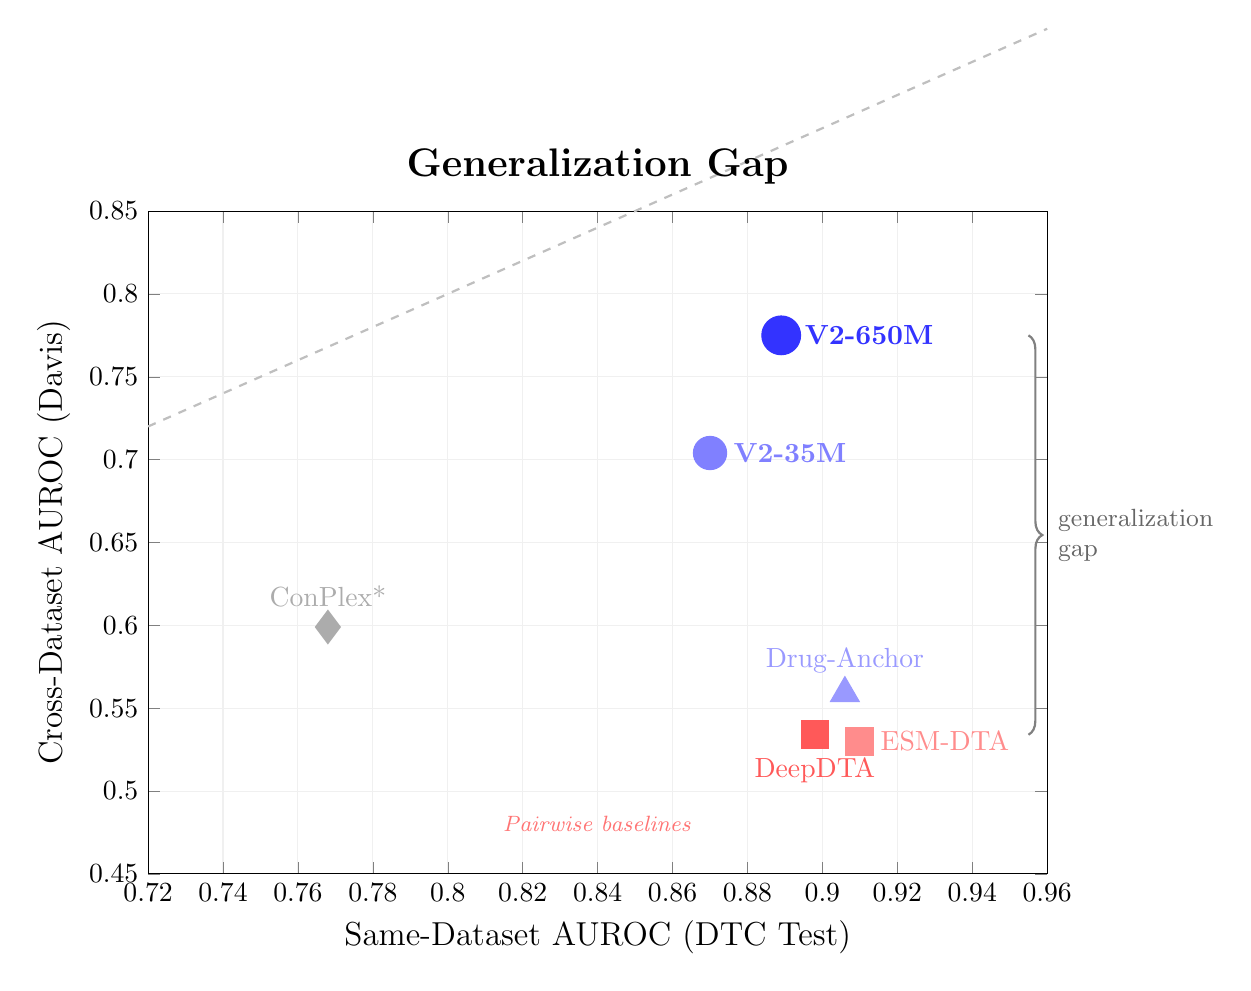
\begin{tikzpicture}
\begin{axis}[
    width=13cm,
    height=10cm,
    xlabel={Same-Dataset AUROC (DTC Test)},
    ylabel={Cross-Dataset AUROC (Davis)},
    xlabel style={font=\large},
    ylabel style={font=\large},
    xmin=0.72, xmax=0.96,
    ymin=0.45, ymax=0.85,
    grid=major,
    grid style={gray!12},
    title={\textbf{Generalization Gap}},
    title style={font=\Large},
    clip=false,
]

% Diagonal: perfect generalization
\addplot[dashed, gray!50, thick, domain=0.72:0.96] {x};

% === Anchor Transfer models (blue tones, circles/triangle) ===
\addplot[only marks, mark=*, mark size=7pt, blue!80] coordinates {(0.889, 0.775)};
\node[right=5pt, font=\normalsize\bfseries, blue!80] at (axis cs:0.889, 0.775) {V2-650M};

\addplot[only marks, mark=*, mark size=6pt, blue!50] coordinates {(0.870, 0.704)};
\node[right=5pt, font=\normalsize\bfseries, blue!50] at (axis cs:0.870, 0.704) {V2-35M};

\addplot[only marks, mark=triangle*, mark size=6pt, blue!40] coordinates {(0.906, 0.559)};
\node[above=4pt, font=\normalsize, blue!40] at (axis cs:0.906, 0.559) {Drug-Anchor};

% === Pairwise baselines (red/gray tones, squares/diamond) ===
\addplot[only marks, mark=square*, mark size=5pt, red!65] coordinates {(0.898, 0.534)};
\node[below=5pt, font=\normalsize, red!65, anchor=north] at (axis cs:0.898, 0.534) {DeepDTA};

\addplot[only marks, mark=square*, mark size=5pt, red!45] coordinates {(0.910, 0.530)};
\node[right=4pt, font=\normalsize, red!45] at (axis cs:0.910, 0.530) {ESM-DTA};

\addplot[only marks, mark=diamond*, mark size=6pt, gray!65] coordinates {(0.768, 0.599)};
\node[above=4pt, font=\normalsize, gray!65] at (axis cs:0.768, 0.599) {ConPlex*};

% Gap annotation brace (outside plot, using clip=false)
\draw[decorate, decoration={brace, amplitude=5pt, mirror}, thick, black!50]
    (axis cs:0.955, 0.534) -- (axis cs:0.955, 0.775)
    node[midway, right=7pt, font=\small, align=left, black!60] {generalization\\gap};

% Grouping label
\node[font=\footnotesize, red!55, align=center] at (axis cs:0.84, 0.48) {\textit{Pairwise baselines}};

\end{axis}
\end{tikzpicture}
\end{document}
